\section{Optimization} \label{sec:implementation}
We employ \theoremref{Thm:supporting_plane} and its discretization eq.\eqref{eq:folding_const} in a simple algorithm to enforce folds along creases while deforming piecewise smooth DOGs. The algorithm tries to minimize an objective, while keeping the DOG constraints and ensuring the formation of folds along all crease curves.

\subsection{Problem setup}
We model our curved folded surfaces as a quad mesh, with a separate connected component for each patch. We denote the set of $n$ mesh vertices in $R^3$ by $V \in R^{n\times3}$, the flattened variables by $\x \in R^{3n}$, and the mesh quad faces by $F$. Each connected component by its own is a DOG, i.e. has the connectivity of a subset of $\Z^2$ and satisfy the DOG angle constraints \cite{rabi18}. The patches themselves also need to align along the creases as detailed at \ref{sec:model} enforced by simple linear constraints as done in \cite{rabi2018shape}. For convenience we call both of these constraints the "DOG constraints" and denote them by $\phi_{d_i}(\x) = 0, 1 \leq i \leq m$.

We are interested in deformations that fold along all creases in a given folding pattern using \theoremref{Thm:supporting_plane} and enforcing eq. \eqref{eq:folding_const}. We enforce these constraints on all crease points, which are points on crease curves that are not crease vertices, besides crease points that have the following degeneracy on the flattened mesh (see \figref{fig:fold_const_degeneracies}):
\begin{enumerate}
	\item Degenerate osculating plane  - Crease points with a curvature smaller than a threshold $k_\eps$. \label{item:deg_osc}
	\item Degenerate edge - Crease points along an edge, splitting it to two parts where one is shorter than $\eps_{r}$\% of the other. \label{item:deg_edge}
	\item Degenerate angle with the intersecting DOG tangent - Crease points where the tangent directions $t_1,t_2$ form an angle with one of the edges $e_f,e_b$ that is smaller than $\eps_\alpha$. \label{item:deg_tan_angle}
\end{enumerate}
Throughout the paper we use the constants $k_\epsilon=1e-5, \eps_r=5\%, \eps_\alpha=3^{\circ}$.

\begin{figure} [h]
	\centering
	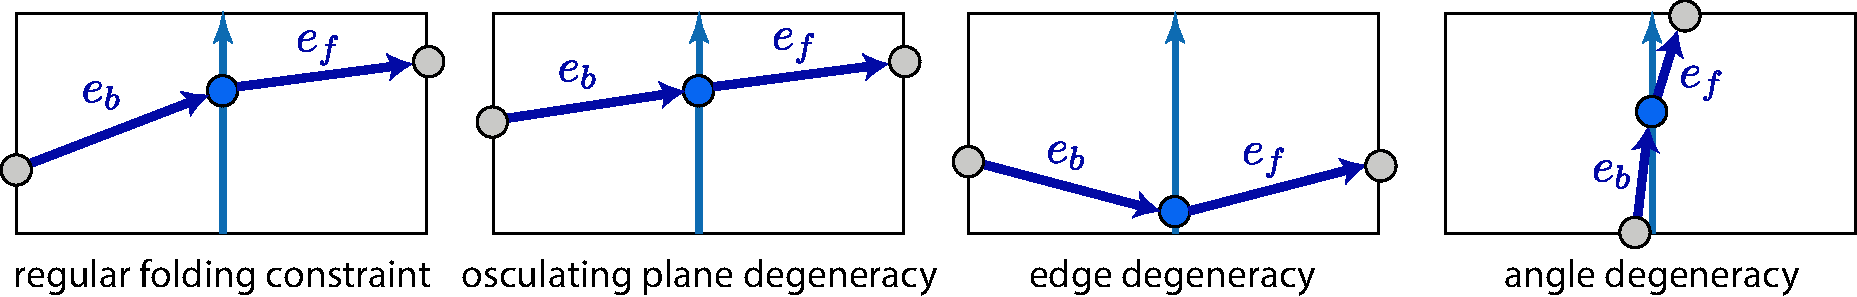
\includegraphics[width=\linewidth]{figures/fold_const_degeneracies}
	\caption{A folding edge constraint defined on a blue crease point splitting the blue edge and degenerate cases where we do not enforce the constraint. From left to right: A regular folding edge constraint, instabilities in the osculating plane's normal as $\frac{e_b \times e_f}{\|e_b \times e_f\|}$ caused by $e_b,e_f$ being almost collinear, degenerate edges as one part of the edge split by the blue crease point is comparably very short, and lastly a very small angle between $e_b$ and the DOG edge crossing the blue point. An angle degeneracy often occurs before or after an edge degeneracy.}
	\label{fig:fold_const_degeneracies}
\end{figure}

The problems we solve in this paper can be written in the form:
\begin{equation} \label{eq:const_opt}
\begin{aligned}
& \argmin_x f(x) \\
& \textrm{subject to} \\
& \phi_{d_i}(\x) = 0, \ \  i = 1, \ldots, m. \\
& \phi_{f_i}(\x) = 0, \ \  i = 1, \ldots, k \\ 
\end{aligned}
\end{equation}
With $f$ as an objective, composed of a weighted sum of a bending objective, isometry objective, positional constraints and other terms as specified in \secref{sec:dog_obj}.

\subsection{Folding constraints}
Motivated by the fact that in the smooth case one cannot move from a folded to a non-folded model around a non-planar point, we strive to always satisfy $\phi_{f_i}(x) = 0$ exactly. The common starting point of a flat surface is an interesting case, as it is a bifurcation point between surfaces satisfying \theoremref{Thm:supporting_plane} and those that do not, which also holds for its discretization \eqref{eq:folding_const_normalized}. To that end we solve our problem with an iterative sequential quadratic programming (SQP) solver with a linesearch, added with two simple strategies to handle the folding constraints $\phi_{d_i}(\x)$:
\begin{enumerate}
	\item Use a penalty term (\cite{nocedal}) punishing on deviation from the constraints. \label{opt:penalty}
	\item Use linesearch method that does not except meshes deviating from the constraints $\phi_{d_i}(\x)$.
\end{enumerate}
As the functions $\text{sgn}(x),H(x)$ involved in the constraints $\phi_{d_i}(\x)$ are not $C^1$, we replace them by the approximations:

\begin{align} 
\begin{split}\label{eq:const_inner}
\text{sgn}(x) \approx \tanh(hx) \\
H(x) \approx  \left\{\begin{array}{@{}l@{\thinspace}l}
0  &: \text{if } x \leq 0, \\
\frac{x^2}{x^2+\delta} &: \text{if } x = 0, \delta > 0 \\\\
\end{array}\right.
\end{split}
\end{align}
using the fixed parameters $h=1000,\delta = 1e-5$. Our approximation for $H(x)$ is taken from by the works of \cite{l0_approximation,autocuts}.  Our use in a homotopy based optimization necessitates an approximation for $H(x)$ that vanishes on a flat mesh, and therefore we do not use the common approximation for the Heaviside function $H(x) \approx \hat{H}(x) =  \frac{1+\tanh(hx)}{2}$ as $\hat H(0) = \frac{1}{2}$.

We refer to the approximated constraints as $\phi^*_i(\x)$. and replace the optimization problem \eqref{eq:const_opt} with the following problem:
\begin{equation} \label{eq:const_opt_penalty}
\begin{aligned}
& \argmin_x f(x) + \alpha \sum \|\phi^*_{f_i}(\x)\|_2^2 \\
& \textrm{subject to} \\
& \phi_{d_i}(\x) = 0, \ \  i = 1, \ldots, m. \\ 
\end{aligned}
\end{equation}
Where $\alpha > 0$ is a metaparameter initialized as $\alpha_0 = 1$, that doubles its value if the linesearch cannot find a point that both decreases a given merit function while satisfying the supporting planes conditions exactly. In practice, the penalty term only affects points that are very close to being planar points, while approaching zero very quickly around already folded points.

\subsection{Equality constrainted SQP}
For ease of notation, we use the following notation to refer to the objective of \eqref{eq:const_opt_penalty}:
\begin{equation}
f_\alpha(\x) = f(x) + \alpha \sum \|\phi^*_{f_i}(\x)\|_2^2
\end{equation}
We minimize \eqref{eq:const_opt_penalty} using an iterative Sequential Quadratic Programming (SQP) solver with a linesearch \cite{nocedal}. Given a set of variables at a given iteration $x^k$ and current values of lagrange multipliers $\lambda^k$, a linesearch equality constrained SQP algorithm iteratively find the next direction for a linesearch of \eqref{eq:const_opt_penalty} by which it sets the next variables $x^{k+1}$ by solving a KKT system of the form:

\begin{equation} \label{eq:KKT_eps}
\begin{gathered}
{K} \begin{pmatrix} d^{k+1} \\ \lambda^{k+1} \end{pmatrix}=\mathbf{b} \\
{K}=\begin{pmatrix}
{\Delta^2_{xx}\mathcal{L}(x^k,\lambda^k)} & {J^\tr}(\x^k)\\
{J(\x^k)} &  0 \\
\end{pmatrix}, \ \ 
\mathbf{b}=\begin{pmatrix}
{\nabla f(x^k)} \\ 
-\phi_{d_i}(x^k)\\
\end{pmatrix}.
\end{gathered}
\end{equation}

Where $J(\x)$ is the Jacobian of the equality constraints in \eqref{eq:const_opt_penalty}, $\Delta^2_{xx}\mathcal{L}(x,\lambda) = H_{f_\alpha}(x)+\sum\lambda_i^{k} \nabla \phi_{d_i}(x)$ is the Lagrangian of the problem and $H_{f_\alpha}(\x)$ is the Hessian of $f_\alpha(\x)$.

Following \cite{rabi2018shape}, we use a minimally modified Jacobian $J^*(x)$ to deal with singularities in DOGs. We also replaced the Hessian of the objective $H_{f_\alpha}(\x)$ by a convex approximation which we denote by $H^*_{f_\alpha}(\x)$, as detailed in \ref{sec:dog_obj}, and thus replace the system \eqref{eq:KKT_eps} by:

\begin{equation} \label{eq:KKT_us}
\begin{gathered}
{K} \begin{pmatrix} d^{k+1} \\ \lambda^{k+1} \end{pmatrix}=\mathbf{b} \\
{K}=\begin{pmatrix}
{ H^*_{f_\alpha}(\x^k)+\sum\lambda_i^{k} \nabla \phi_{d_i}(\x^k)} & {J^{*^\tr}(\x^k)}\\
{J^*(\x^k)} &  0 \\
\end{pmatrix}, \ \ 
\mathbf{b}=\begin{pmatrix}
{\nabla f(x^k)} \\ 
-\phi_{d_i}(x^k)\\
\end{pmatrix}.
\end{gathered}
\end{equation}

We note that at \cite{rabi2018shape} the authors discretized Laplacian metric flows by solving a similar system with a Laplacian instead of the objectives' Lagrangian, however we found that replacing the Laplacian by the Lagrangian followed by convexifying the Hessian performs significantly better, especially on larger models. As common in SQP algorithms, our linesearch used a merit function defined as a combination of the objective and the constraints, thus the linesearch chooses step sizes that both reduce the objective and keep the constraints numerically feasible. This removed the need of the slower LBFGS constraints projection used by \cite{rabi18,rabi2018shape}. We used the L2 merit function \cite{nocedal}:
\begin{equation}
\psi(\x;\mu) = f_\alpha(\x)+\mu\sum\|\phi_{d_i}(x)\|_2
\end{equation}
where we update the parameter $\mu^k$ at each iteration using the absolute values of the Lagrange multipliers \cite{nocedal}:
\begin{equation}
\max(c_\mu \max(\{\abs{\lambda_i^k}\}), \mu_0)	
\end{equation}
with $c_\mu = 1.1$ and $\mu_0 = 0.05$.

\subsection{Objectives and constraints} \label{sec:dog_obj}
\MiR{Mean curvature is quadratic under isometry (or even under same ratio, similar to Wardetzky's observance but true for the shape2018 paper as well), then iso energy (convex hessian). Then positional edge/point constraints by linear constraints (which are sometimes build as a curve constrained flow by slowly interpolating it). Then dihedral angle and fold bias are all written down as constraints and used as a quadratic objective with a Gauss-newton hessian. They also all start with zero deviation.}